\documentclass[a4paper,11pt, twoside]{article}

%%%%%%%%%%%%%% Predefined packages
\usepackage{times,amsmath,eurosym, amssymb, color, graphicx}
\usepackage{booktabs, cellspace}
\usepackage{hyperref}
\usepackage[export]{adjustbox}
\usepackage{float}
\usepackage{amsthm}
%%%%%%%%%%%%%% Packages: IF YOU NEED TO ADD A PACKAGE, PLEASE DO IT HERE:

%%%%%%%%%%%%%% Useful definitions
\newcommand{\R}{\mathbb R}
\newcommand{\C}{\mathbb C}
\newcommand{\F}{\mathbb F}
\newcommand{\Z}{\mathbb Z}
\newcommand{\Q}{\mathbb Q}
\newcommand{\N}{\mathbb N}
\newcommand\veczwo[2]{\left[\begin{array}{r}#1\\#2\end{array}\right]}
\newcommand\vecdrei[3]{\left[\begin{array}{r}#1\\#2\\#3\end{array}\right]}
\newcommand\vecdreic[3]{\left[\begin{array}{c}#1\\#2\\#3\end{array}\right]}
\newcommand\vecvier[4]{\left[\begin{array}{r}#1\\#2\\#3\\#4\end{array}\right]}
\newcommand\vecsechs[6]{\left[\begin{array}{r}#1\\#2\\#3\\#4\\#5\\#6\end{array}\right]}
\newcommand\matzz[4]{\left[\begin{array}{rr}#1&#2\\#3&#4\end{array}\right]}
\newcommand\matdd[9]{\left[\begin{array}{rrr}#1&#2&#3\\#4&#5&#6\\#7&#8&#9\end{array}\right]}
\newcommand\matddc[9]{\left[\begin{array}{ccc}#1&#2&#3\\#4&#5&#6\\#7&#8&#9\end{array}\right]}
%%%%%%%%%%%%%%% 

%%%%%%%%%%%%% Page layout
\topmargin-20mm
\headheight10mm
\headsep10mm
\topskip0.1mm
\hoffset-15mm
\textwidth15.5cm
\textheight22cm
\parindent0em
%\markleft{\authors}
%\markright{\shorttitle} 
\pagenumbering{arabic}
%%%%%%%%%%%%%%%%%%

%%%%%%%%%%%%%%%%%%%%%%%%%%%%%%%
\begin{document}
\thispagestyle{empty}
\hrule
$\vphantom{i}$ \\[-.25cm]
\section{Cryptographical Hash Functions:\newline Collision Resistance And Padding}  
$\vphantom{i}\hspace{.65cm}$  \textit{Thomas Heinrichs | StudID: 79430}
$\vphantom{i}$ \\[-.25cm]
\hrule
%%%%%%%%%%%%%%%%%%%%%%%%%%%%%%%%%%%%%%

%%%%%%%%%%%%%%%%%%%%%%%%% USE SUBSECTION AND SUB-SUBSECTION ONLY
\subsection*{Abstract}
This paper aims to introduce the fundamental idea behind cryptographical hash functions. Starting with the real world application areas of hash functions, the reader will gain an idea about the security requirements of those. These requirements will be explained more precisely in the next paragraph together with the concept of a cryptographical hash function. This concept will lead to the term of collision resistance which needs to be defined properly. Following up a short outlook about key derivation functions is given. In the next section of this paper the need of padding will be presented. In the end the results will be summed up shortly and the challenges of writing this paper will be shown. 


\subsection{Fundamental idea behind hash functions and real world application areas}
In general hash functions have an input of arbitrary length bit strings $m$ and generate an output $o$ which is called digest, hash-code or hash-value. The digest should have the following characteristics: 
\begin{itemize}
	\setlength\itemsep{0pt}
	\item The output seems to be pseudo-randomly. If message $m$ is altered, output $o$ changes in a way that it seems to be unpredictable.
	\item The hashed value in output $o$ needs to be efficient, so it is computed fast .
	\item Hash functions need to be deterministic. The output $o$ will be the same each time the message $m$ will be used as input. 
	\item It needs to be an one-way-function. It shouldn't be possible to compute the message $m$ out of output $o$ (irreversible).
	\item A hash function needs to be collision resistant. It should be hard to find different input messages $m$ which result in the same output $o$.
\end{itemize}
The meaning of these items in a mathematical way, will be discussed later on. To show the different application areas of hash functions these properties are sufficient.\newline

There is a various number of possibilities to use hash functions. Below is a list with the most important ones: 
\begin{itemize}
    \item In software development it is essential to use one of those to \textbf{secure user related information} stored in the database. By adding a salt to the plain-text before using a hash function, the data is stored safely, even if an attacker has gained access to the database. For instance hashed passwords still can be used for authentication later on, since only the hashed values are compared.
    \item A \textbf{message digest} is another application area of hash functions. This is a fixed size numeric representation of a message which is achieved by applying a hash function upon it. After encrypting the message digest it can be used as a digital signature. This digital signature is sent with the message itself, so the receiver can calculate the digest himself to prove its integrity. If the message changed during transmission, the digest is going to change too, which can be detected within the receiver. If a message digest is using a secret symmetric key for encryption it is known as Message Authentication Code (MAC). \cite{message_digest}
    \item Another technology which is based upon hash functions is the \textbf{block-chain}. Quickly explained, the block-chain encodes transactions into a block of digital data which is uniquely signed or identified. Each of these blocks is connected to one another which creates a irreversible, immutable chain. With that construct, it can be prevented, that any of those blocks is altered, or another block is inserted between two existing blocks. Especially for the digital signature and the identification hash functions are used. \cite{blockchain}
\end{itemize}
These three application areas show how crucial hash functions are to those technologies and can be seen as motivation for the rest of this paper. How to build a secure cryptographical hash function and the mathematical ideas are explained in the next chapter. 


\subsection{Cryptographical hash functions}
A standard hash function which deals with arbitrary length bit strings and generates a digest is not equal to a cryptographical one. In the next step the necessary "must-haves" are introduced. \newline\\[0.1cm]
When we are talking about a cryptographical hash function, it needs to be at least one-way. Therefore a string $y$ from co-domain of the domain $H$ and a value $x$ in $H$ is given. To achieve a one way function the expression
\begin{align*}
    H(x)=y
\end{align*}
needs to be computationally infeasible. A hash function is computationally infeasible, if a function calculating the preimage for a hash function producing an output of $t$ $bit$ would require a time of $O(2^t)$.\newline\\[0.1cm]
This context can be visualised in a so called security game. They are used to define security for cryptographical components. These games are quite abstract and played between an attacker or adversary and a challenger. The attacker needs to achieve some objective given with the information from the challenger or the environment. In the security games the adversary is listed as a box and the challenger at the outside of the box. The security game for a one-way function is shown in figure \ref{fig:secgame_onewayfunc}.
\begin{figure}[H]
	\centering
	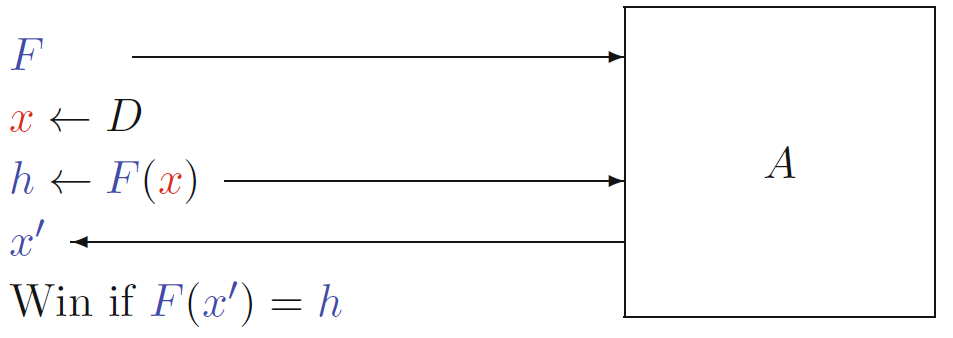
\includegraphics[scale=0.34]{figures/SecGame_OneWayFunc.png}
	\caption{Security game for one-way functions from Nigel P. Smarts book}
	\label{fig:secgame_onewayfunc}
\end{figure}
A hash function is also said to be a one-way hash function (OWHF) if it is second preimage resistant.\cite{Preneel2005}\newline\\[0.1cm]
It's also necessary that cryptographical hash functions are preimage and second preimage resistant. That means it should be hard to find two different message strings $m$ and $m'$, such that the digits are equally $H(m') = H(m)$. "Second preimage resistance is also known as weak collision resistance." \cite{Preneel2005} To achieve second preimage resistance a cryptographical hash function with $t$ $bit$ must require at least $2^t$ queries before an attacker can find a second preimage. This results into about a length of at least 80 bits (in 2004).\cite{Preneel2005}. In contrast the advantage of the adversary $A$ to break second preimage resistance of a function $H$ needs to be about $\frac{1}{2^t}$ or even smaller.\newline
Mathematically it can be expressed as: 
\begin{align*}
    Adv_H^{2nd\ Preimage} (A) = Pr[A\ wins\ the\ 2nd-preimage\ game]
\end{align*}
The advantage measures how successful an attack of the hash function is, distinguishing it from an idealised version of this type function.\cite{advantage}\newline\\[0.1cm]
After introducing second preimage resistance, or so called week collision resistance, we are going to have a look upon "real" collision resistance. Therefore we need to consider a function $H$ which maps elements in a domain $D$ to a co-domain $C$. The domain $D$ is a set of arbitrary length bit strings and is much larger than the co-domain. A function is called collision resistant if it is infeasible to find two distinct values such that:
\begin{align*}
    H(m) = H('m)
\end{align*}
But there is a problem regarding how security is defined. In this case we can assume that something is secure if the probability of winning the security game is very small.\newline
Since it is known that domain $D$ is bigger than out co-domain $C$ there must exist such a pair that $H(m) = H('m)$. By using a hash function from a family of functions the attacker will not know which function was selected ahead of time. Summed up Nigel P. Smart defines collision resistance like this:
\newtheorem{mydef}{Definition}
\begin{mydef}
    A function H is said to be collision resistant by human ignorance if it is believed to be infeasible to write down a collision for the function, i.e. two elements in the domain mapping to the same element in the co-domain.
\end{mydef}
As shown in the birthday paradox, building a hash function featuring collision resistance is harder than building one-way hash function. 
\begin{figure}[H]
	\centering
	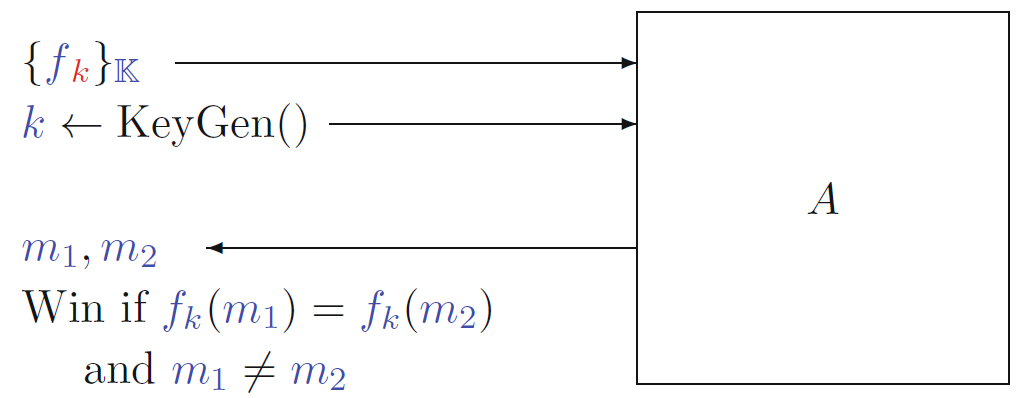
\includegraphics[scale=0.34]{figures/SecGame_CollisionResistance.png}
	\caption{Security game for collision resistance of a family of functions from Nigel P. Smarts book}
	\label{fig:secgame_collisionresistance}
\end{figure}
Since using multiple functions provides a better security and is a possible solution to the problem mentioned earlier, figure \ref{fig:secgame_collisionresistance} illustrates the security game for collision resistance of a family of functions.


\subsection{Key Derivation Functions (KDF)}
An application field of hash function which was introduced previously are Key Derivation Functions (KDF's). This function derives cryptography keys from a password and must deal with arbitrary length inputs and outputs. \cite{key_derivation_function}\newline
Mathematically expressed the KDF $G_k$ takes a variable key size $_k$ and derives $l \in \mathbb N$ keys. In figure \ref{fig:secgame_kfd} the security game for KDF's is visualised. This introduction gives a short overview of this topic. More detailed knowledge can be worked out independently. 
\begin{figure}[H]
	\centering
	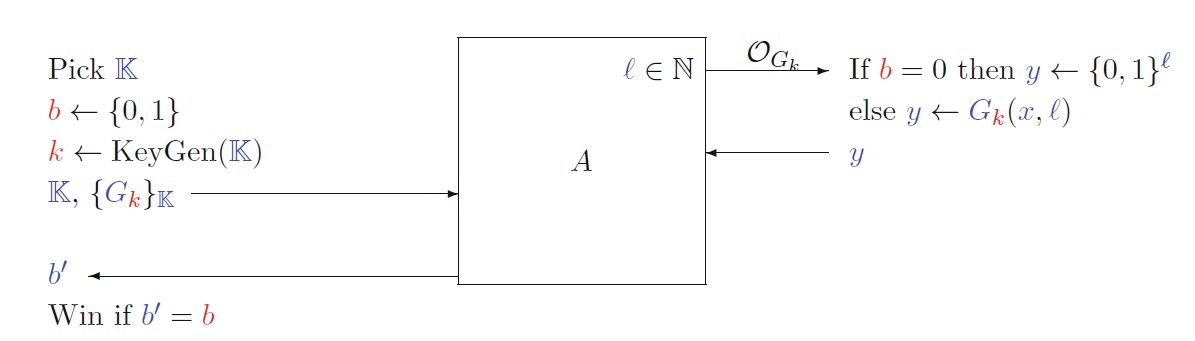
\includegraphics[scale=0.5]{figures/SecGame_KDF.png}
	\caption{Security game for the Key Derivation Function introduced above from Nigel P. Smarts book}
	\label{fig:secgame_kfd}
\end{figure}


\subsection{Padding in hashed messages}
This last chapter of this paper is going to show the importance of padding and why it is used. Afterwards we will have a look upon some padding schemes.\newline\\[0.1cm]
To be able to deal with arbitrary length strings in hash functions we need to pad a message. Our simple function has got a fixed length input or an input with the multiple of a fixed length. The fixed length is called the block size. When applying such a padding scheme, the message will be edited by adding bits onto the message. By applying this method every message will fit into our hash function.\newline\\[0.1cm]
Whether you pad at the beginning, in the middle or at the end doesn't matter. But in practice it is common to extend the message at the end.
To apply padding functions, some variables need to be introduced. The input message $m$ has a length of $l$ bit and the block size equals $b$ bits. The $i$ in the formulas shown in figure \ref{fig:padding_schemes} refers to the padding scheme which is used. There are many possible padding schemes. The following list shows a few samples.
\begin{figure}[H]
	\centering
	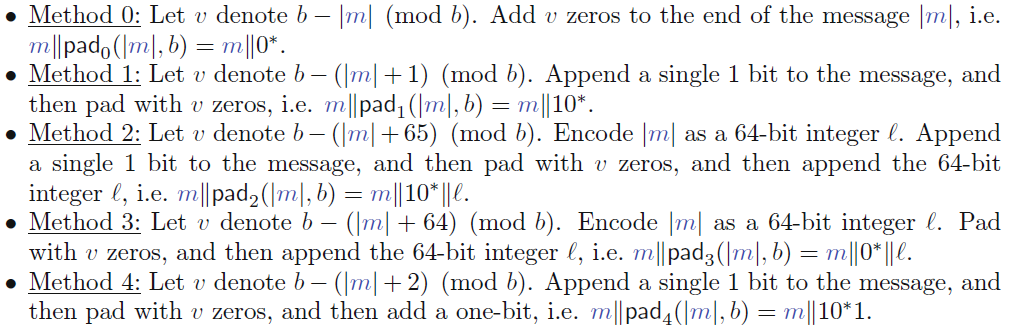
\includegraphics[scale=0.6]{figures/Padding_Schemes.png}
	\caption{Padding schemes as described in Nigel P. Smarts book}
	\label{fig:padding_schemes}
\end{figure}
For the first method it is not possible to reverse the padded message into the original message. For all other methods this would be easily possible. 


\subsection{Conclusion}
This paper has shown the idea behind cryptographical hash function and some real world application areas were introduced. The mathematical ideas behind preimage- and collision- resistance have been explained. The reader has also gained an insight into key-derivation-functions and padding. These ideas, defining how to build a good cryptographical hash function, will be used in the next chapters, in which some concrete hashing algorithms will be introduced. In the next paragraph there will be a short reflection about the challenges of writing this paper.\newline\\[0.1cm]
Due to the time limited presentation it was necessary to adapt and shorten this paper. The result is a superficial overview upon the topic of cryptographical hash functions and padding. My intention was to pick out the basic ideas and explain them. The difficulty was to work out the scattered information from several chapters. For instance it was necessary to have a look at security games and block ciphers. The information written in those chapters was crucial to my paper.\newline
In the end I hope that the theory behind hash function and padding has been understood well and it can be used for further chapters about this topic.


%%%%%%%%%%%%%%%%%%%%%%%%%%%%%%%%%%%%%%%%%%%%%% End of Contribution
\bibliography{bibliography}
\bibliographystyle{alphadin}
%%%%%%%%%%%%%%%%%%%%%%%%%%%%%%%%%%% 
\end{document}